\section{Traditional Machine Learning}

\subsection{Feature Generation}

To extract features, we firstly converted all images to grayscale. Then, we 
considered the following image features:


% \begin{figure}[t]
% \centering

% \caption{Confusion matrix for binary-classification }
% \label{cmbin}
% \end{figure}

We showed the changes of the average training accuracy under different numbers of PCA 
components in \figref{pcamulti} in both settings. 




\begin{figure}[t]
\centering
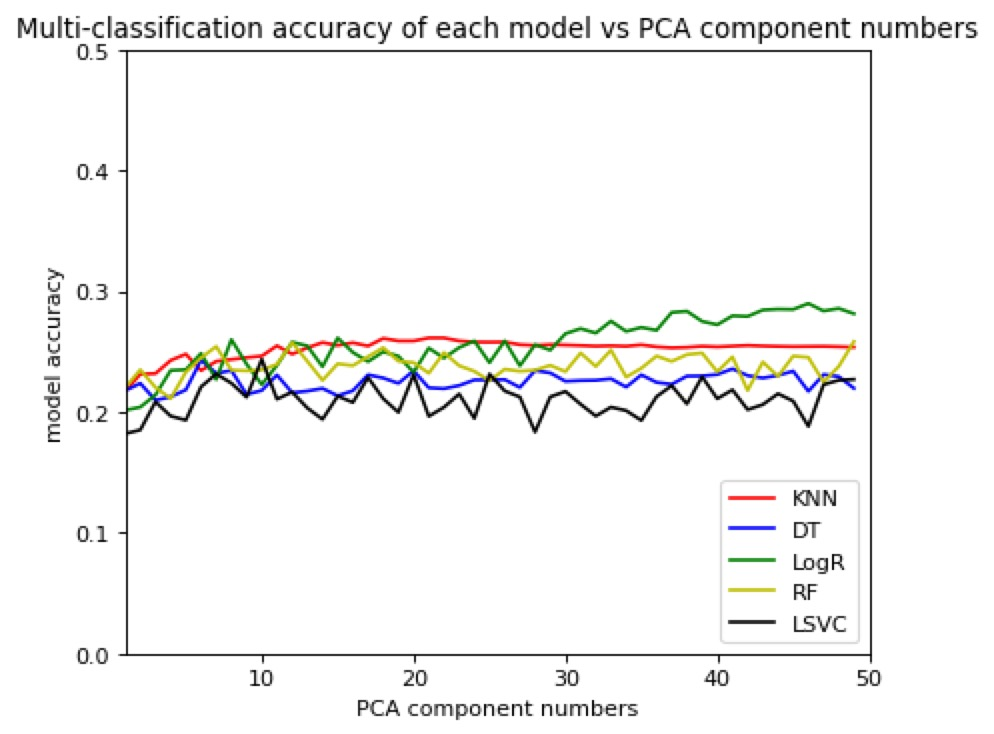
\includegraphics[width=0.4\textwidth]{multi_class.jpeg}
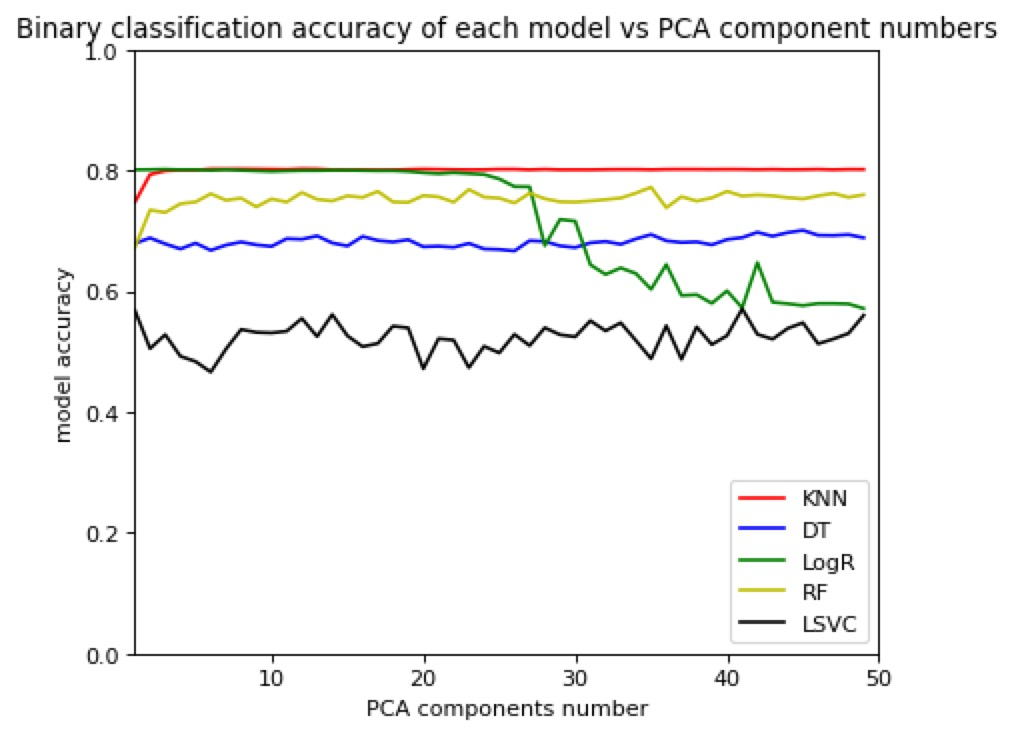
\includegraphics[width=0.4\textwidth]{binrary_class.jpeg}
\caption{Training accuracy of selected models vs. PCA component numbers in 
multi-classification (left) and binary-classification (right)}
\label{pcamulti}
\end{figure}
% \begin{figure}[t]
% \centering
% 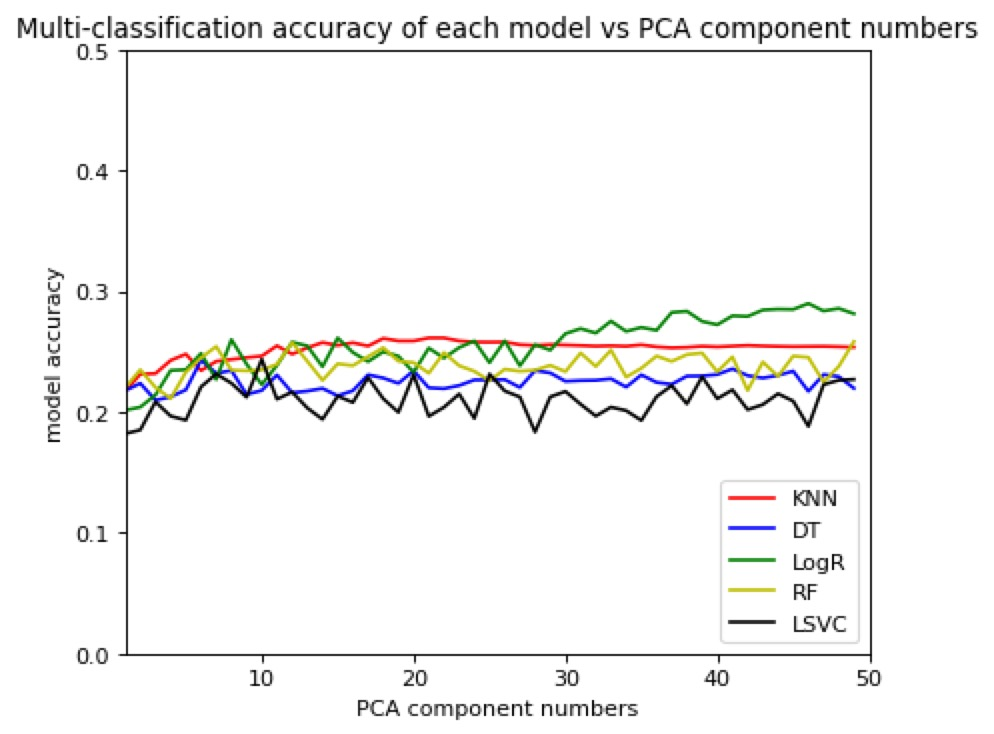
\includegraphics[width=0.4\textwidth]{multi_class.jpeg}
% \caption{Multi-classification accuracy of each model vs PCA component numbers}
% \label{pcamulti}
% \end{figure}

% \begin{figure}[t]
% \centering
% 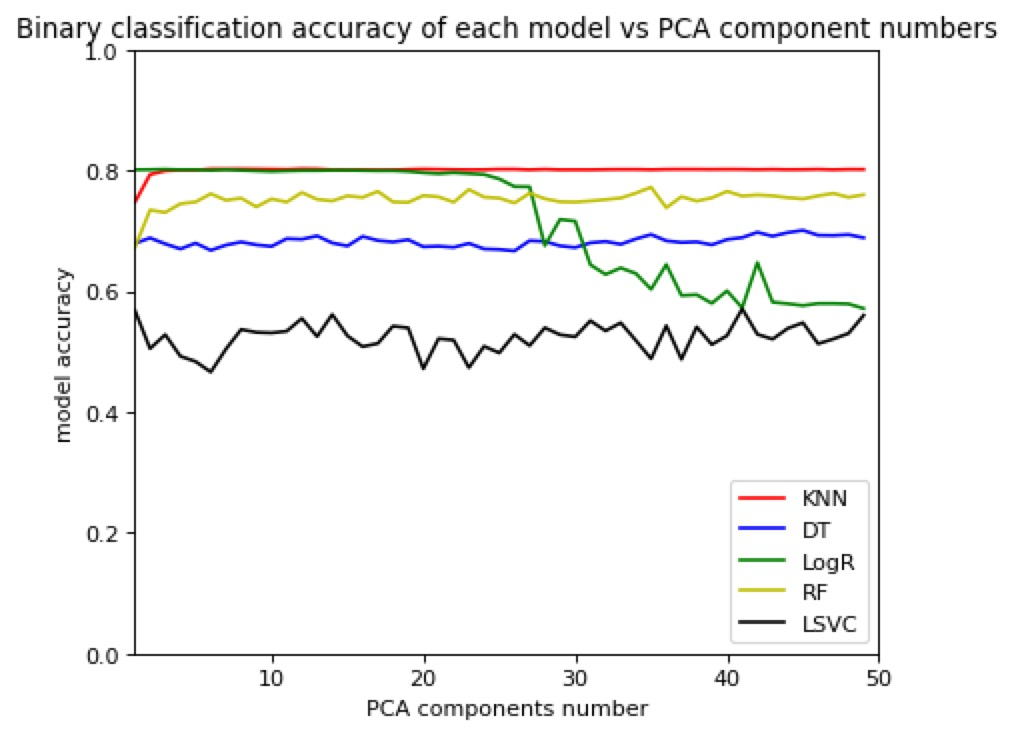
\includegraphics[width=0.4\textwidth]{binrary_class.jpeg}
% \caption{Binary-classification accuracy of each model vs PCA component numbers}
% \label{pcabin}
% \end{figure}

\begin{itemize}
\item Histogram of Pixels (HP): the distribution of pixel values (i.e., the number of pixels of the same value), which resulted in 256-dimension feature vector. 
\item Histogram of oriented gradients (HOG): used to detect the object. It counts occurrences of gradient orientation in localized portions of an image. This method produced a 64-dimension feature vector~\cite{hog}.
\item Haralick Texture (HAK): a feature matrix that counts the co-occurrence of neighboring gray levels in the image. It is used to quantify an image based on texture. This matrix has the dimension of gray levels N in the region of interest (ROI). We generated a 13-dimension feature vector using this method~\cite{haralick}.
\item Local Binary Patterns (LBP): summarizes the local structure in an image by comparing each pixel with its neighborhood. If the intensity of the center pixel is greater or equal to its neighbor, then denote it with 1 and vice versa. This method results in a 20-dimension features vector~\cite{lbp}. 
\item Parameter-Free Threshold Adjacency Statistics (PFTAS): the distribution of white pixels that have zero to N neighbors. In this project, we used the built-in python library Mahotas to build a 54-dimensional PFTAS-feature vector~\cite{pftas}.
\item Image moments: the weighted average of the image pixels intensity. It is useful for catching image properties. 
We applied two different ways, Zernike Moments (ZM) and Hu moments (HU), to obtain a 32-dimension feature vector~\cite{zm,hu}.
\item Scale-Invariant Feature Transform (SIFT): SIFT is an algorithm for detecting and describing 
local features in images. We generated a 2,048-dimension feature vector using it~\cite{sift}. 	
\end{itemize}

All features have been shown to be sufficient under various settings in the image classification tasks. Note that the standard way to identify diabetic retinopathy 
severity level is to examine the blood vessels, microaneurysms, and exudates in 
the retina~\cite{1,2,3}. Our goal is to use those image recognition and objection detection algorithms  
to catch these characteristics of retina. We finally extract 2,497 features from for each image. In the next session we performed 
feature dimension reduction to filter out important features from the 2497 features. 	

\begin{figure}[t]
\centering
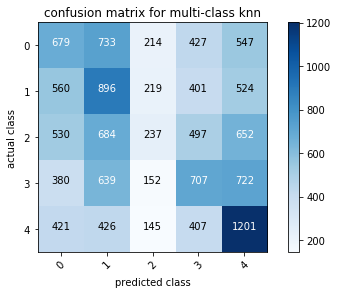
\includegraphics[width=0.35\textwidth]{multi.png}
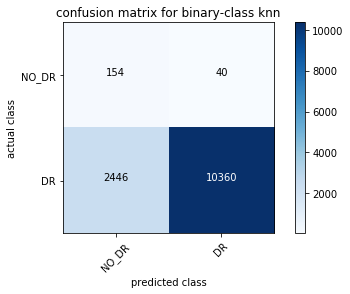
\includegraphics[width=0.35\textwidth]{binary_knn.png}
\caption{Confusion matrices of KNN 
in multi-classification~(left) and logistic regression in binary-classification(right) }
\label{cmmulti}
\end{figure}

\subsection{Model Selection}

The model selection pipeline is as follows: firstly apply PCA to all the features using $m$ as the PCA component number; then, for a given model $m$ and the model parameter $p$, train a classifier on the training set with 10-fold CV, and record the average classification accuracy. That means to explore every possible combinations of ($n$, $m$, $p$), and select the setting that produce the highest accuracy. 

The number of PCA components $n$ we have tested ranging from 1 to 50. We considered the following seven conventional ML models: CART decision tree, extra tree, KNN,  SVM, logistic regression, random forest, and AdaBoost with decision tree.  For binary classifiers, we used the one-vs-rest strategy, which is the most commonly used strategy for multiclass classification.  We trained one classifier for each of the classes against all the other classes (i.e., class as positive and all the other classes as negatives), and vote the output that has the highest confidence score as the class for a given test sample. We fixed the parameters being used for most of the models based on the suggestions from Sklearn, except for KNN. For KNN, we varied the number of neighbors from 1 to 30. 

\subsection{Evaluation}
We considered two settings: 
\begin{itemize}
\item Multiclass classification: classify an image based on its severity level 0 -- 4. 
\item Binary classification: label an image as \texttt{NoDR} or \texttt{DR}, with all the images of severity 1 -- 4 been considered as \texttt{DR} and severity 0 as \texttt{NoDR}. Binary classification is more commonly discussed in literatures. 
\end{itemize}

\begin{figure}[t]
\centering
%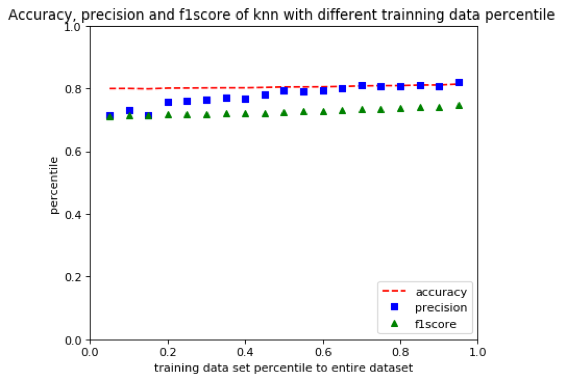
\includegraphics[width=0.4\textwidth]{accuracy.png}
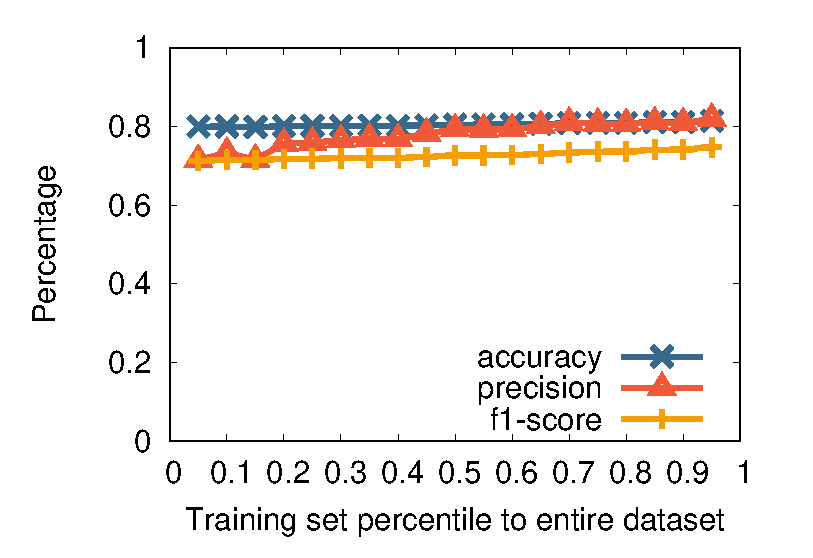
\includegraphics[width=0.4\textwidth]{knn.eps}
\caption{Accuracy, precision and f1-score of KNN with different training data percentile }
\label{knnacc}
\end{figure}


\begin{figure}[t]
\centering
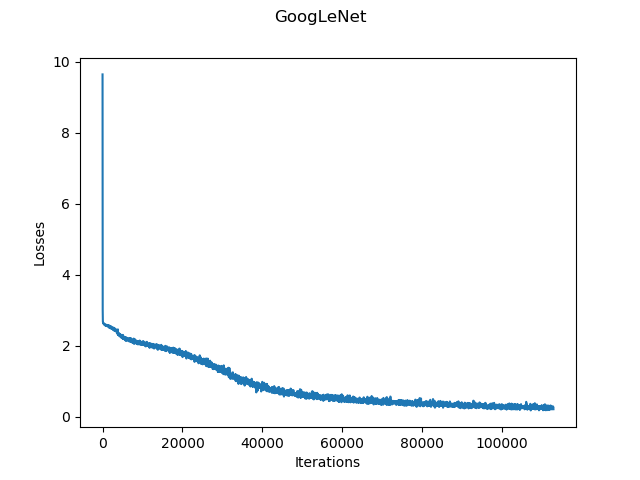
\includegraphics[width=0.35\textwidth]{google_loss.png}
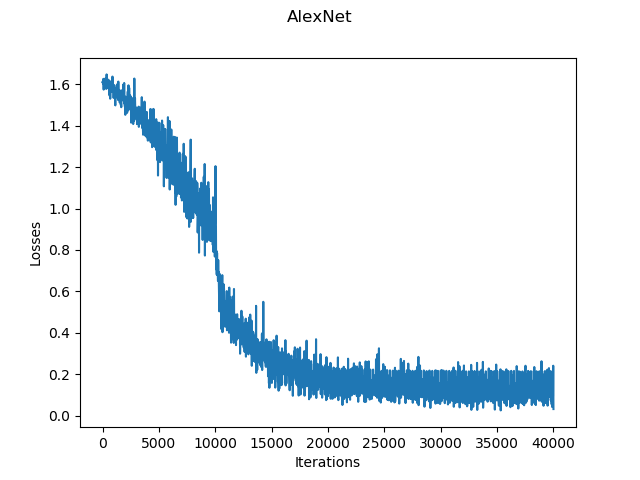
\includegraphics[width=0.35\textwidth]{alex_loss.png}
\caption{Loss vs. iteration numbers for GoogLeNet and AlexNet}
\label{cnn_loss}
\end{figure}

\subsubsection{Multiclass setting}
The logistic regression model produced the highest accuracy, 28.98\%, when $n = 46$. Unfortunately, none of the models produced more than 30\% accuracy. We then repeated the model selection procedures multiple times and see consistent results:  logistic regression with $n = 45$ or $n = 46$ gives 
the highest accuracy $\approx$ 30\%. 

We applied this best model to the test dataset and the resulting accuracy is 28.62\%. This is 
just slightly better than random guessing for 5-class classification. 
The confusion matrix is shown in \figref{cmmulti}. 

\subsubsection{Binary setting}
In binary setting, KNN with 22 neighborers produced the highest accuracy when 
$n = 20$, and the corresponding accuracy on test set is 80.19\%. The confusion matrix is shown in \figref{cmmulti}. For comparison, 
we also tested the other models against the test set, and found indeed the selected 
KNN model gave the best performance: the other models only have 50\% to 78\% 
accuracy on the test set. Surprisingly, SVM with non-linear kernels, which is 
the default choice and has been considered as one of the most effective setting in many prior image 
classification works, perform poorly this time,even worsen than SVM with linear kernels. 

We further examined how would the test accuracy 
changes under different train/test set splits with fixed parameter settings. As shown in \figref{knnacc} 
the weighted test accuracy, precision, and f1-score increases as the training set 
size increases. However, even using a small training dataset, KNN still produces a 
more than 70\% accuracy on testing dataset, which is much better than the best accuracy 
SVM can achieve.  

We show how training accuracy changes under different PCA component numbers in~\figref{pcamulti}. The series represent different machine learning 
algorithms. For a given algorithm, we fixed the parameters as the best-performing 
ones among all testings. As we can see, the accuracy for most algorithms 
are almost the same as the number of PCA components increases. The training 
accuracy of logistic regression are comparable to KNN when PCA component 
number $<$ 25, but decreased quickly as PCA component number went up. 
We didn't test larger PCA component numbers as doing so might be conflict with the idea of dimension reduction. 
One idea is to use deep neural networks to generate more representative features 
as the inputs to our machine learning classifiers. We would like to examine 
this idea in the future.

\section{Discussion}
Our experiments suggest the traditional machine learning models perform poorly 
for identifying the severity level based on retina images, using generic image 
features. However, to simply diagnose if a person has DR or not, the traditional 
models work, and have relatively better accuracy. Unfortunately, the performance 
of our models are still worsen than some of the prior works~\cite{1,2,3}, which used ML with  
retina-specific features, such as diameter of optic disk, microaneurysms, 
and exudates. Nevertheless, our results indicate that ML with  
generic images features are capable, to some extent, to catch 
characteristics of domain-specific images. 





